\documentclass[a4paper, 12pt]{article}
\usepackage{mathtools}
\usepackage{bm}
\usepackage{tikz}
\setlength{\parindent}{0cm}
\setlength{\parskip}{12pt plus4mm minus3mm}

\begin{document}
\section{The motion of the polhode}
Given a rigid rotating object, with angular momentum $L$ and kinetic energy $T$, let us work in a rotating reference frame moving with the object. In that frame we will use Cartesian co-ordinates aligned with the three principal axes of the moment of inertia of the object.

In those co-ordinates let the angular velocity vector $\bm{\omega}$ have components $\omega_1, \omega_2,\omega_3$. The moment of inertia tensor $\bm{I}$ has the form:

$$
I = \begin{pmatrix}
I_1 & 0 & 0 \\
0   & I_2 & 0 \\
0 & 0 & I_3 \\  
\end{pmatrix}
$$

We will assume all principal axes are distinct and that (for the sake of argument) $I_1 < I_2 < I_3$. We will refer to the unit vectors in this co-ordinate system as $\bm{n_1}, \bm{n_2}, \bm{n_3}$.

The inertia tensor may be visualised using an ellipsoid. In 3D space, consider the surface traced out by the vector $\bm{x}$ subject to the constraint $\bm{x}\cdot\bm{I}\cdot\bm{x} = 1$. This is an ellipsoid with equation $$I_1x^2 + I_2y^2 + I_3z^2 = 1$$

For fixed angular momentum (in a situation where there is no torque) $\bm{I}\cdot\bm{\omega}$ is constant and hence the magnitudes of $I$  and $\omega$ are inversely proportional. Kinetic energy is given by $\frac{\bm{I}\cdot\bm{\omega}^2}{2}$. It will be at a minimum where $\omega$ is least and hence when $I$ is largest, which is when the axis of rotation is pointing in the direction of $\bm{n_3}$. Similarly the energy is at a maximum where the axis of rotation is pointing in the direction of $\bm{n_1}$.

Informally, for the same angular momentum, reducing the moment of inertia about an axis will proprtionately increase the angular velocity. The kinetic energy depends will decrease linearly with the moment of inertia (because the mass of the object is closer in and so less of it is rotating at the higher speeds on the outer edge of the object) but increase as the square of the angular velocity. The result is that the lower the moment of inertia, the higher the kinetic energy for any given angular momentum.

Exactly the same reasoning shows that the situation is the other way around when considering possible angular moment for constant kinetic energy. The minimum angular momentum will be in the direction of $\bm{n_1}$ and the maximum in the direction of $\bm{n_3}$.

This, and many other things, should be clearer if we may consider two ellipsoids traced out by the angular velocity vector:
\begin{itemize}
\item The {\bf energy ellipsoid} or {\bf Poinsot's ellipsoid}, representing a surface of constant kinetic energy. This is congruent to the inertia ellipsoid but scaled up by a factor of $T$.
  \begin{equation}\label{eq:energy_ellipsoid}
    I_1\omega_1^2 + I_2\omega_2^2 + I_3\omega_3^2 =T
  \end{equation}
\item The {\bf momental ellipsoid}, representing a surface of constant angular momentum. This will in general have a different shape from the inertia ellipsoid.
  \begin{equation}\label{eq:momental_ellipsoid}
    I_1^2\omega_1^2 + I_2^2\omega_2^2 + I_3^2\omega_3^2 = L^2
  \end{equation}
\end{itemize}

In the general case of distinct principal axes of the moment of inertia tensor that we are considering these two ellipsoids will be different shapes. The energy ellipsoid's maximum and minimum lengths will be along the first and third axes respecitvely, whereas the momental ellipsoid will bulge the other way, with the third axis being the longest and the first shortest.

%A specific example may help. The Swan Vesta matchbox is particularly well suited to angular momentum problems because of its dimensions which are:
%
%\begin{center}
%  \begin{tabular}{l l}
%    height & 17.4mm \\
%    width & 47.68mm \\
%    depth & 79.37mm \\
%  \end{tabular}
%\end{center}
%
%Assuming a mass of roughly $16g$ and a thickness of the box of mm this would give us a moment of inertia tensor (in $\textup{kgcm}^2$) of
%
%$$
%I=
%\begin{pmatrix}
%  1279 & 0 & 0 \\
%  0 & 1788 & 0 \\
%  0 & 0 & 2122 \\
%\end{pmatrix}
%$$

By setting $\omega_1=1$ and $\omega_2=\omega_3=0$ in (\ref{eq:momental_ellipsoid}) we can find the maximum value of the moment of inertia for fixed kinetic energy $T$ and a similar operation find the mimimum:

\begin{eqnarray*}
  I_1T \leq L^2 \leq I_3 T \\
  L^2=I_1T & \textrm{at} & \mathbf{\omega}=(\sqrt{\frac{T}{I_1}}, 0, 0) \\
  L^2=I_3T & \textrm{at} & \mathbf{\omega}=(0, 0, \sqrt{\frac{T}{I_3}}) \\
\end{eqnarray*}

We shall consider only the situation where there is no external turning force (torque) and no loss of energy (dissipation) both $L^2$ and $T$ are constants. The polhode is constrained to move on the intersection of the two ellipsoids, which will be a single 1-dimensional path in the general case.

To help visualise this, we will work with the energy ellipsoid (though exactly the same approach would work for the momental ellipsoid). Consider the projection of the energy ellipsoid onto the plane normal to the first principal axis. The path of the particle can be obtained by eliminating $\omega_1$ from the ellipsoid equations by subtracting $I_1(\ref{eq:energy_ellipsoid})$ from $(\ref{eq:momental_ellipsoid})$.

\begin{align}
  (I_2^2 - I_1I_2)\omega_2^2 + (I_3^2-I_1I_3)\omega_3^2 & = L^2 - I_1T
\end{align}

Because $I_1$ is smaller than both $I_2$ and $I_3$ the coefficients of $\omega_1$ and $\omega_2$ are both positive. The RHS is also positive because $L^2 > I_1T$. This is the equation of an ellipse.


\begin{center}
  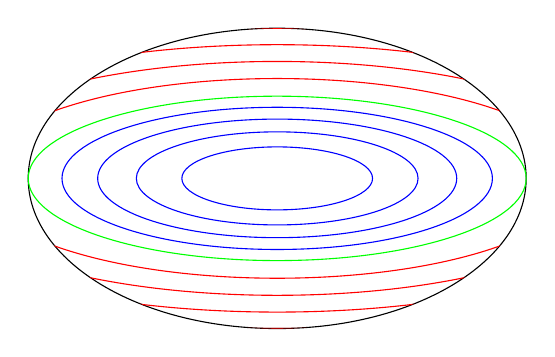
\begin{tikzpicture}%[yscale=1.8]%[scale=3]
    \draw [black] (0, 0) ellipse (3.162cm and 1.907cm);
\draw [blue] (0, 0) ellipse (0.000cm and 0.000cm);
\draw [blue] (0, 0) ellipse (1.211cm and 0.400cm);
\draw [blue] (0, 0) ellipse (1.789cm and 0.591cm);
\draw [blue] (0, 0) ellipse (2.280cm and 0.753cm);
\draw [blue] (0, 0) ellipse (2.733cm and 0.903cm);
\draw [green] (0, 0) ellipse (3.162cm and 1.044cm);
\begin{scope}
\clip (0, 0) ellipse (3.162cm and 1.907cm);
\draw [red] (0, 0) ellipse (3.841cm and 1.268cm);
\draw [red] (0, 0) ellipse (4.497cm and 1.485cm);
\draw [red] (0, 0) ellipse (5.140cm and 1.698cm);
\draw [red] (0, 0) ellipse (5.774cm and 1.907cm);
\end{scope}

    %\draw [black] (0, 0) ellipse (4.472cm and 2.697cm);
    %\draw [blue] (0, 0) ellipse (0.000cm and 0.000cm);
    %\draw [blue] (0, 0) ellipse (1.936cm and 0.640cm);
    %\draw [blue] (0, 0) ellipse (2.887cm and 0.953cm);
    %\draw [blue] (0, 0) ellipse (3.708cm and 1.225cm);
    %\draw [blue] (0, 0) ellipse (4.472cm and 1.477cm);
    %\begin{scope}
    %  \clip(0, 0) ellipse(4.472cm and 2.697cm);
    %  \draw [green] (0, 0) ellipse (5.431cm and 1.794cm);
    %  \draw [green] (0, 0) ellipse (6.360cm and 2.100cm);
    %  \draw [green] (0, 0) ellipse (7.269cm and 2.401cm);
    %  \draw [green] (0, 0) ellipse (8.165cm and 2.697cm);
    %\end{scope}
  \end{tikzpicture}
\end{center}

\section{Dynamics of the polhode}

Euler's equations for the rotation of the object in this co-ordinate system are:

\begin{align}
  I_1\dot{\omega_1}& =(I_2 - I_3)\omega_2\omega_3 \label{eq:euler1} \\
  I_2\dot{\omega_2}& =(I_3 - I_1)\omega_2\omega_3 \\
  I_3\dot{\omega_3}& =(I_1 - I_2)\omega_2\omega_3 
\end{align}

We can use equations \ref{eq:momental_ellipsoid} and \ref{eq:energy_ellipsoid} to express two of the components of $\boldsymbol{\omega}$ in terms of the third.

Subtracting $I_2$ times equation \ref{eq:energy_ellipsoid} from \ref{eq:momental_ellipsoid} we obtain:
\begin{equation}
  (I_1^2 - I_1I_2)\omega_1^2 + (I_3^2 - I_2I_3)\omega_3^2 = L^2 - I_2T
\end{equation}

Rearranging in terms of $I_3$ we have:

\begin{align}
  I_3^2 &=\frac{L^2 - I_2T - (I_1^2 - I_1I_2)\omega_1^2}{I_3^2 - I_2I_3} \\
  I_3 &=\sqrt{\frac{L^2 - I_2T - (I_1^2 - I_1I_2)\omega_1^2}{I_3^2 - I_2I_3}}
\end{align}

And using the same arguments we can express $I_2$ as:

\begin{equation}
  I_2 =\sqrt{\frac{L^2 - I_3T - (I_1^2 - I_1I_3)\omega_1^2}{I_2^2 - I_2I_3}}
\end{equation}


Inserting both of these into the first of Euler's equations (equation \ref{eq:euler1}) gives us:

\begin{equation}
  I_1\dot{\omega_1} = \sqrt{\frac{L^2 - I_2T - (I_1^2 - I_1I_2)\omega_1^2}{I_3^2 - I_2I_3}}\sqrt{\frac{L^2 - I_3T - (I_1^2 - I_1I_3)\omega_1^2}{I_2^2 - I_2I_3}}
\end{equation}

This may be rearranged to:

  \begin{align}
    \dot{\omega_1} &= \sqrt{\frac{1}{I_1(I_3^2 - I_2I_3)(I_2^2 - I_2I_3)}}\sqrt{L^2 - I_2T - (I_1^2 - I_1I_2)\omega_1^2}\sqrt{L^2 - I_3T - (I_1^2 - I_1I_3)\omega_1^2} \\
    \dot{\omega_1} &= \sqrt{\frac{(L^2 - I_2T)(L^2 - I_3T)}{I_1(I_3^2 - I_2I_3)(I_2^2 - I_2I_3)}}\sqrt{ 1 - \frac{I_1^2 - I_1I_2}{L^2 - I_2T}\omega_1^2}\sqrt{ 1 - \frac{I_1^2 - I_1I_3}{L^2 - I_3T}\omega_1^2}\label{eq:fullode}
  \end{align}

Let

\begin{align}
  y^2 &= \frac{I_1^2 - I_1I_2}{L^2 - I_2T}\omega_1^2 \\
  \dot{y} &= \frac{I_1^2 - I_1I_2}{L^2 - I_2T}\dot{\omega_1} \\
\end{align}

And let
\begin{align}
  k^2 & = \frac{(I_1^2 - I_1I_3)(L^2 - I_2T)}{(L^2 - I_3T)(I_1^2 - I_1I_2)} \\  
\end{align}

Then equation \ref{eq:fullode} becomes:
\begin{align}
  \dot{y}&=\frac{(I_1^2 - I_1I_3)(L^2 - I_2T)}{(L^2 - I_3T)(I_1^2 - I_1I_2)}\sqrt{\frac{(L^2 - I_2T)(L^2 - I_3T)}{I_1(I_3^2 - I_2I_3)(I_2^2 - I_2I_3)}}\sqrt{ 1 - y^2}\sqrt{ 1 - k^2y^2}
\end{align}

This is a straightforward ODE to transform into an integral, giving us:
\begin{align}
  t + C &=\frac{(I_1^2 - I_1I_3)(L^2 - I_2T)}{(L^2 - I_3T)(I_1^2 - I_1I_2)}\sqrt{\frac{(L^2 - I_2T)(L^2 - I_3T)}{I_1(I_3^2 - I_2I_3)(I_2^2 - I_2I_3)}}\int\frac{1}{\sqrt{ 1 - y^2}\sqrt{ 1 - k^2y^2}}
\end{align}

\end{document}
